\documentclass{standalone}

\usepackage{graphicx}
\usepackage{caption}
\usepackage{tikz}
\usetikzlibrary{positioning,shapes.symbols,matrix}

\begin{document}

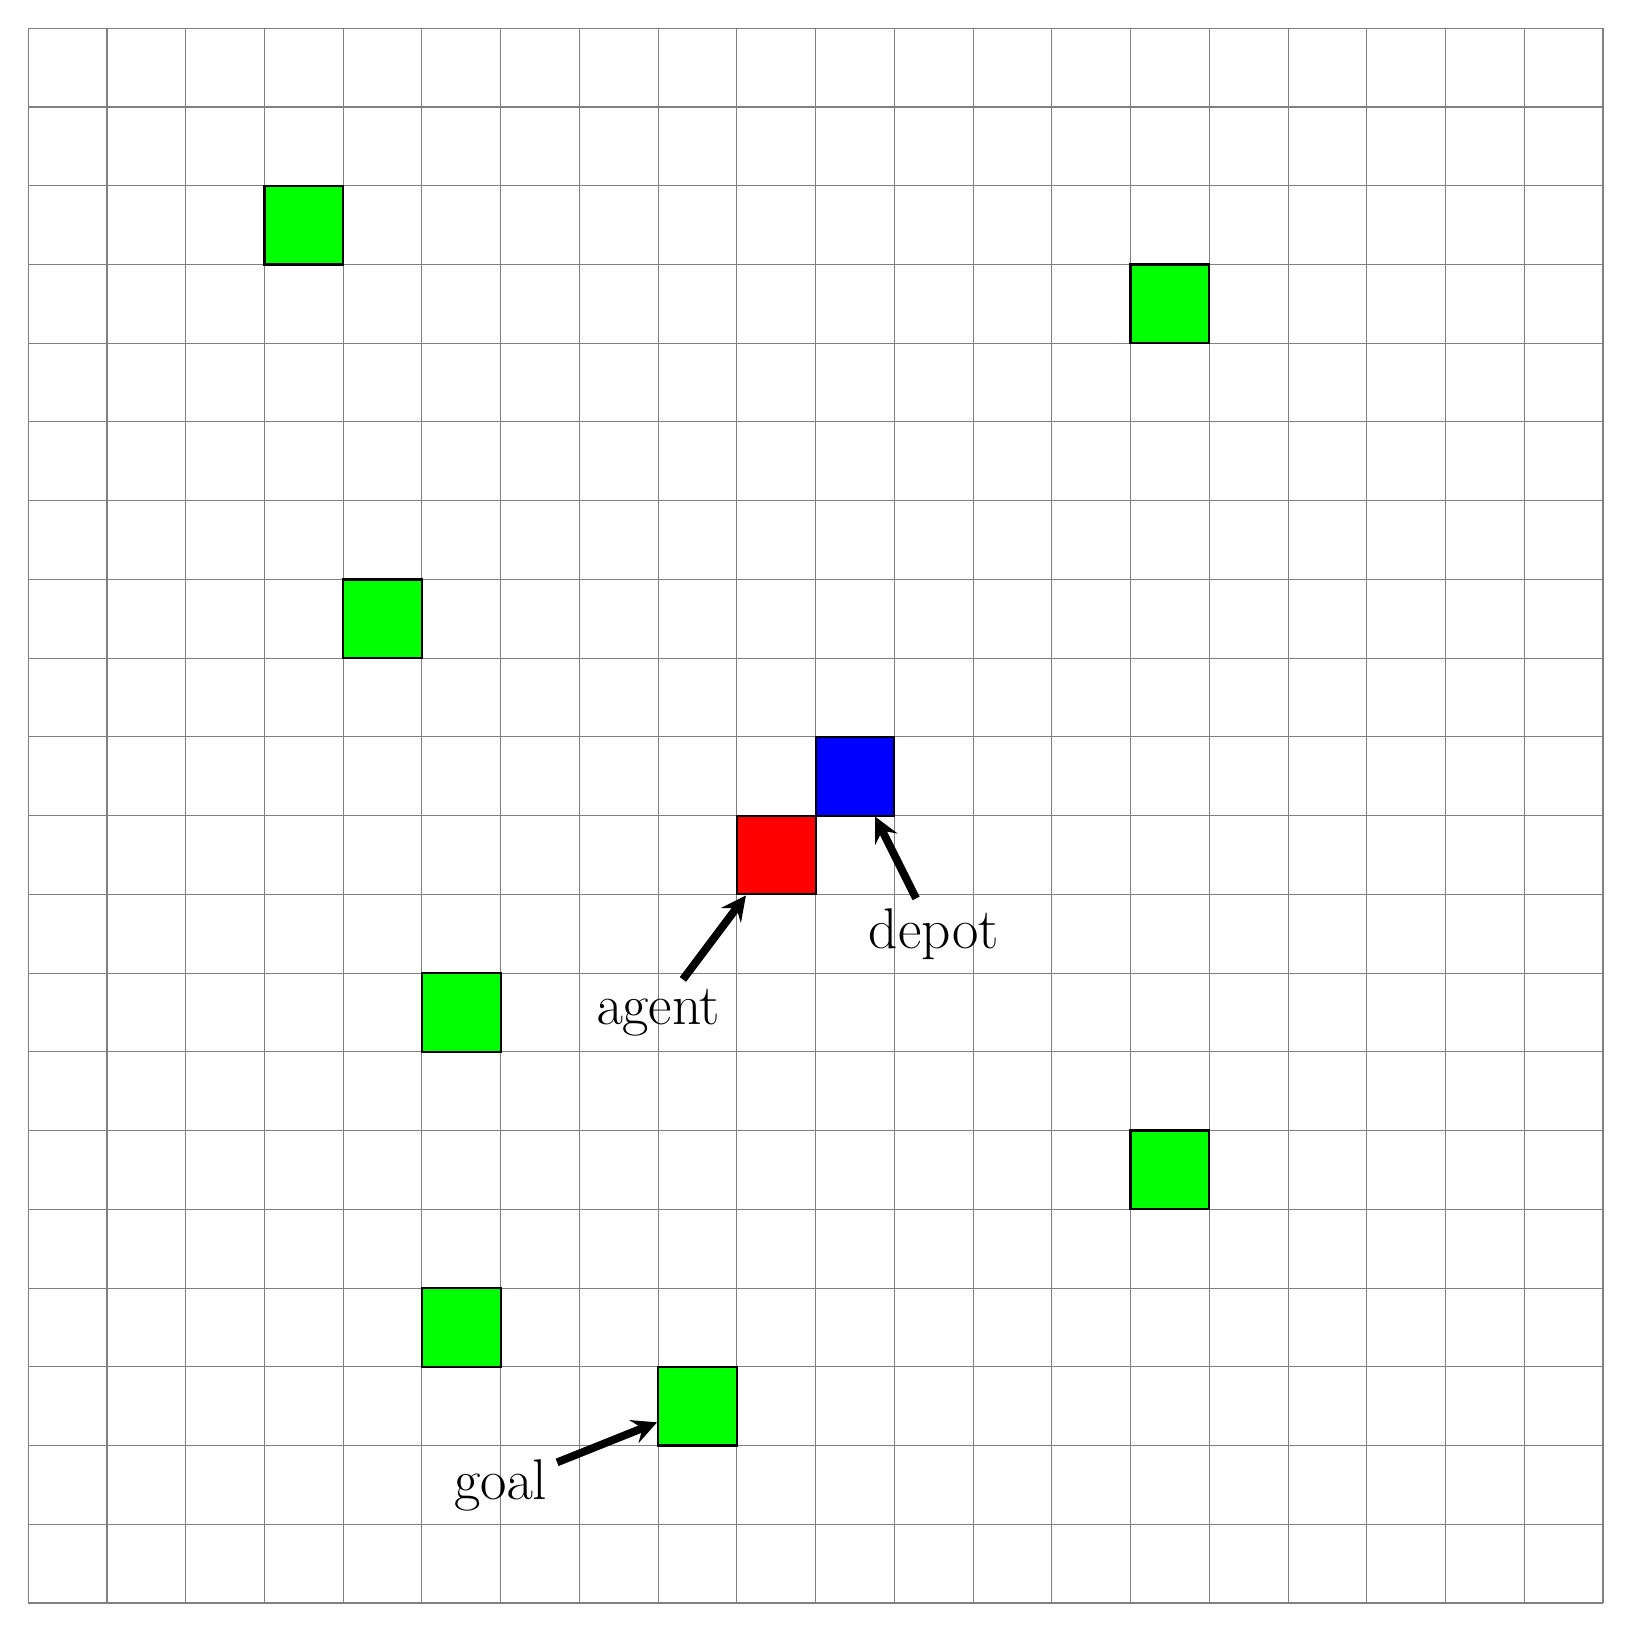
\begin{tikzpicture}
    [%%%%%%%%%%%%%%%%%%%%%%%%%%%%%%
    box/.style={rectangle,draw=black,thick, minimum size=1cm},
    ]%%%%%%%%%%%%%%%%%%%%%%%%%%%%%%

    \draw[step=1cm,color=gray] (0,0) grid (20,20);


    % agent
    \node[box,fill=red] at (9.5,9.5)(agent){};
    \node at (8,7.5) (agent_text) {\huge{agent}};
    \draw [-stealth,line width=0.1cm](agent_text) -- (agent);

    % depot
    \node[box,fill=blue] at (10.5,10.5)(depot){};
    \node at (11.5,8.5) (depot_text) {\huge{depot}};
    \draw [-stealth,line width=0.1cm](depot_text) -- (depot);

    % goal
    \node[box,fill=green] at (8.5,2.5)(goal){};
    \node at (6,1.5) (goal_text) {\huge{goal}};
    \draw [-stealth,line width=0.1cm](goal_text) -- (goal);
    \node[box,fill=green] at (5.5,3.5) {};
    \node[box,fill=green] at (5.5,+7.5) {};
    \node[box,fill=green] at (4.5,+12.5) {};
    \node[box,fill=green] at (14.5,+16.5) {};
    \node[box,fill=green] at (14.5,+5.5) {};
    \node[box,fill=green] at (3.5,+17.5) {};

\end{tikzpicture}

% \begin{tikzpicture}
%     % [%%%%%%%%%%%%%%%%%%%%%%%%%%%%%%
%     % box/.style={signal,draw,signal,to=south},
%     % ]%%%%%%%%%%%%%%%%%%%%%%%%%%%%%%
%     \node[draw,circle,minimum size=0.5cm] {drink water}
%         child {node[draw,rectangle] {fridge water}
%             child{node{go to fridge}}
%             child{node{take the water}}
%             child{node{drink the water}}
%         }
%         child {node [red] {child 2} edge from parent [blue] node [right, brown] {x}};
% \end{tikzpicture}
\end{document}